\documentclass[11pt]{article}
\usepackage[margin=3cm]{geometry}
\usepackage[italian]{babel}
\usepackage[hidelinks]{hyperref}
\usepackage{amsmath}
\usepackage{graphicx}
\usepackage[nameinlink, noabbrev, capitalise, italian]{cleveref}
\usepackage{enumitem}
\usepackage{caption}
\usepackage{float}
\usepackage{amsmath}
\usepackage[ruled, vlined, linesnumbered]{algorithm2e}
\SetAlgorithmName{Algoritmo}{Algoritmo}{Elenco degli algoritmi}
\crefname{algocf}{Algoritmo}{Algoritmo}
\usepackage{array}
\usepackage[bottom]{footmisc}

\tolerance=1
\emergencystretch=\maxdimen
\hyphenpenalty=10000
\hbadness=10000
\setlength\parindent{0pt}

\def\gmaps{\textit{Google Maps}}

\begin{document}
\begin{titlepage}
    \begin{center}
        \vspace*{5cm}
            
        \Huge
        \textbf{Wave Map}\\
        \huge
        \textbf{Cellular Connectivity and Noise Map}
            
        \vspace{0.5cm}
        \LARGE
        Relazione
            
        \vspace{1cm}
          
		\hfill
		\begin{center}
        	{\large{\bf Xia $\cdot$ Tian Cheng}}\\[-0.2em]
			{\large Matricola: \texttt{0000975129}}\\[-0.2em]
			{\large Email: tiancheng.xia@studio.unibo.it}
        \end{center}
            
        \vspace{4cm}
            
        Anno accademico\\
        $2022 - 2023$
            
        \vspace{0.8cm}
            
            
        \Large
        Corso di Laboratorio di applicazioni mobili\\
        Alma Mater Studiorum $\cdot$ Università di Bologna\\
            
    \end{center}
\end{titlepage}
\newpage

\pagenumbering{roman}
\tableofcontents
\newpage

\pagenumbering{arabic}


\section{Introduzione}

\subsection{Feature implementate}

Le feature implementate dall'applicazione sono le seguenti:
\begin{itemize}
    \item Mappa suddivisa in aree non sovrapposte con ridimensionamento automatico delle celle in base al livello dello zoom (\cref{fig:overview_map}).
    \item Range della qualità delle misurazioni calcolato automaticamente, con possibilità di scegliere il numero di classi da creare (\cref{fig:overview_ranges}).
    \item Misurazione di Wi-Fi, LTE, Bluetooth e suono con le seguenti modalità:
    \begin{itemize}[topsep=0pt]
        \item Attiva: su comando dell'utente.
        \item Passiva: dopo un determinato intervallo temporale o durante il movimento. 
        \item In background: durante il movimento.
    \end{itemize}
    \item Filtro di ricerca per alcune tipologie di misurazioni (Wi-Fi e Bluetooth) (\cref{fig:query}).
    \item Notifiche per aree prive di misurazioni recenti.
    \item Esportazione su file e importazione delle misurazioni (\cref{fig:overview_import_export}).
    \item Gestione del tema chiaro/scuro e lingue (italiano e inglese).
\end{itemize}


\subsection{Screenshot applicazione}

\begin{figure}[H]
    \centering
    \begin{minipage}[b]{0.25\textwidth}
      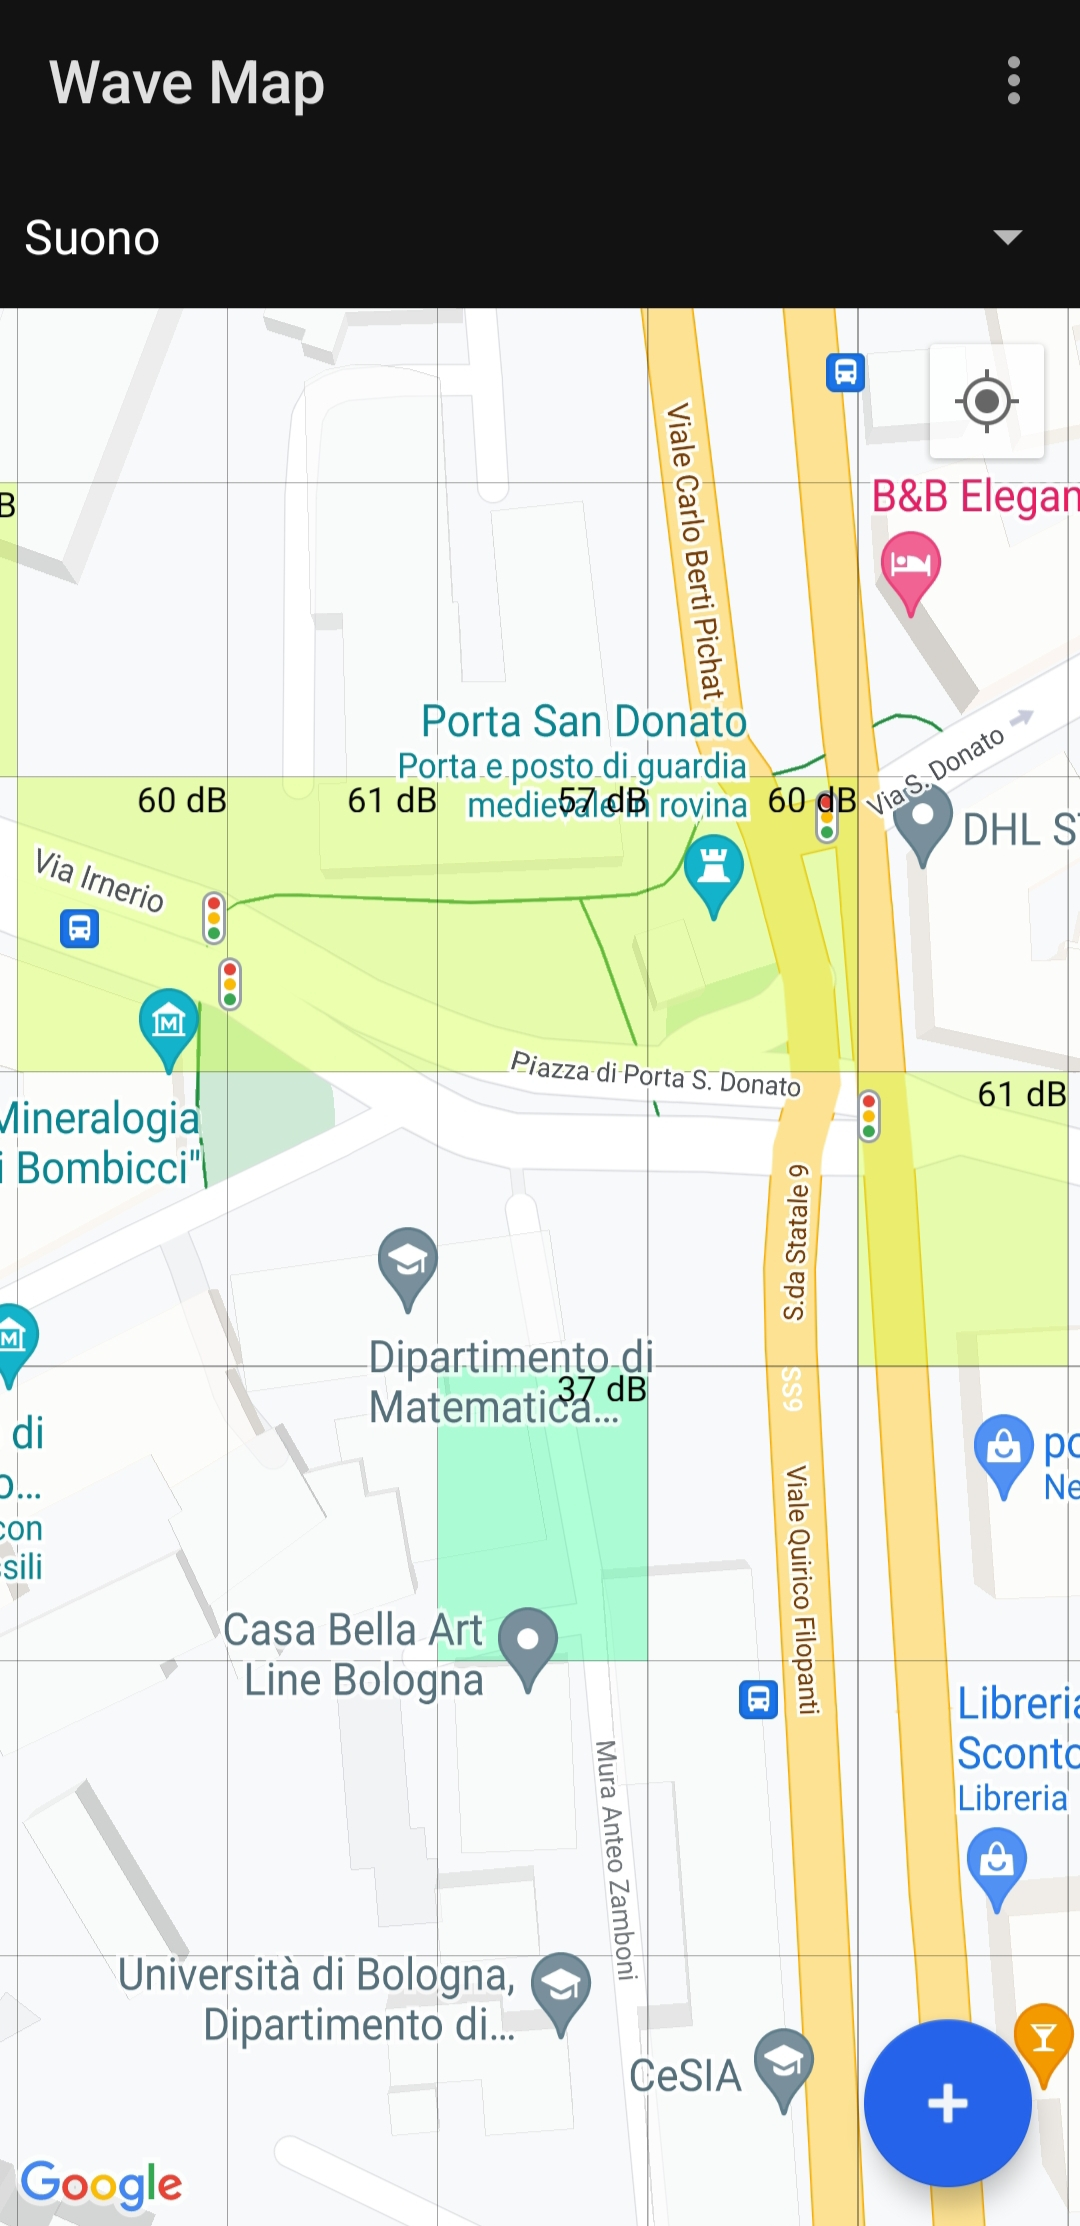
\includegraphics[width=\textwidth]{./img/overview/map_zoom1.jpg}
    \end{minipage}
    \hspace*{1cm}
    \begin{minipage}[b]{0.25\textwidth}
      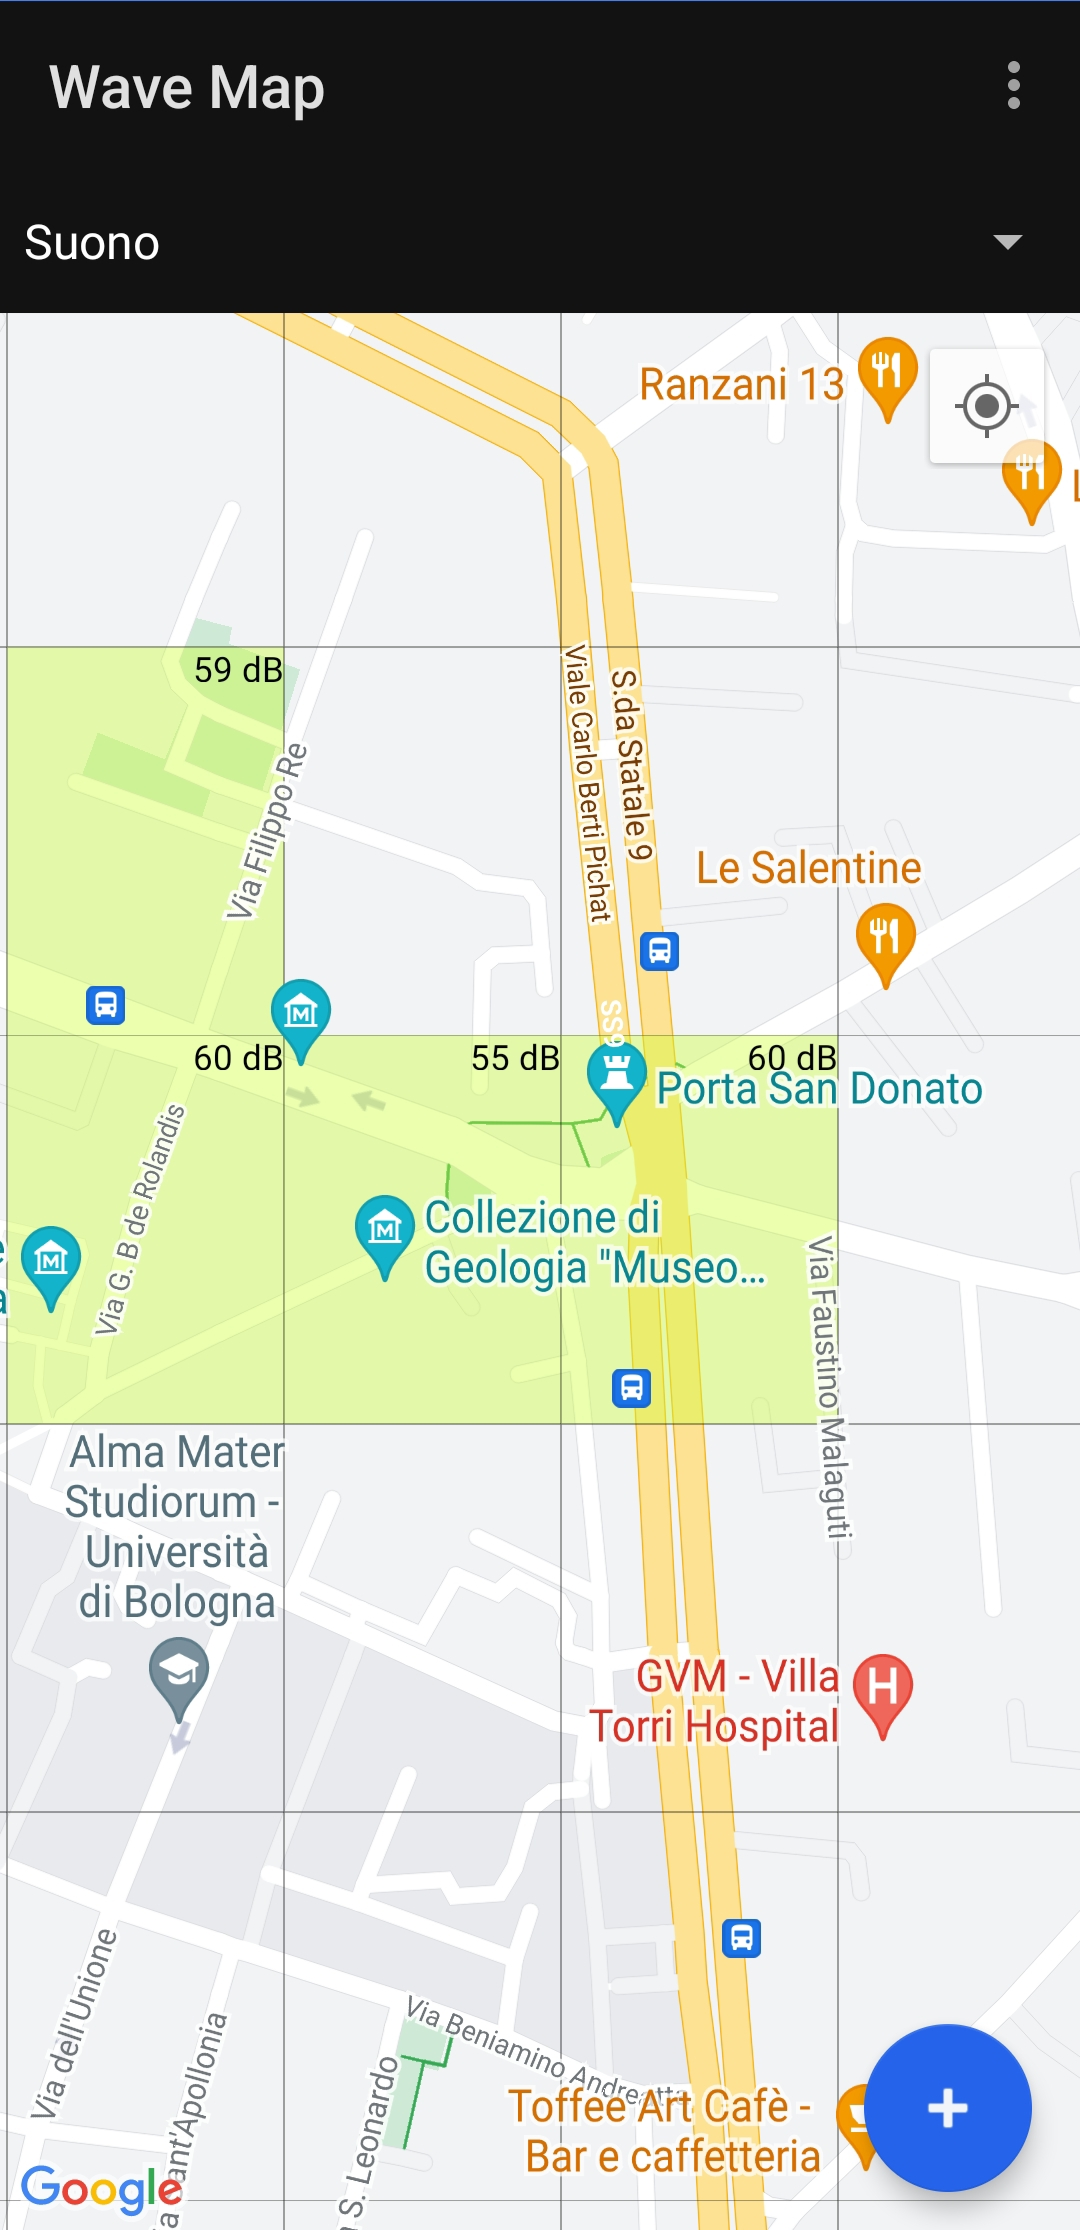
\includegraphics[width=\textwidth]{./img/overview/map_zoom2.jpg}
    \end{minipage}
    \caption{Mappa con celle ridimensionate in base al livello di zoom} \label{fig:overview_map}
\end{figure}

\begin{figure}[H]
    \centering
    \begin{minipage}[b]{0.25\textwidth}
      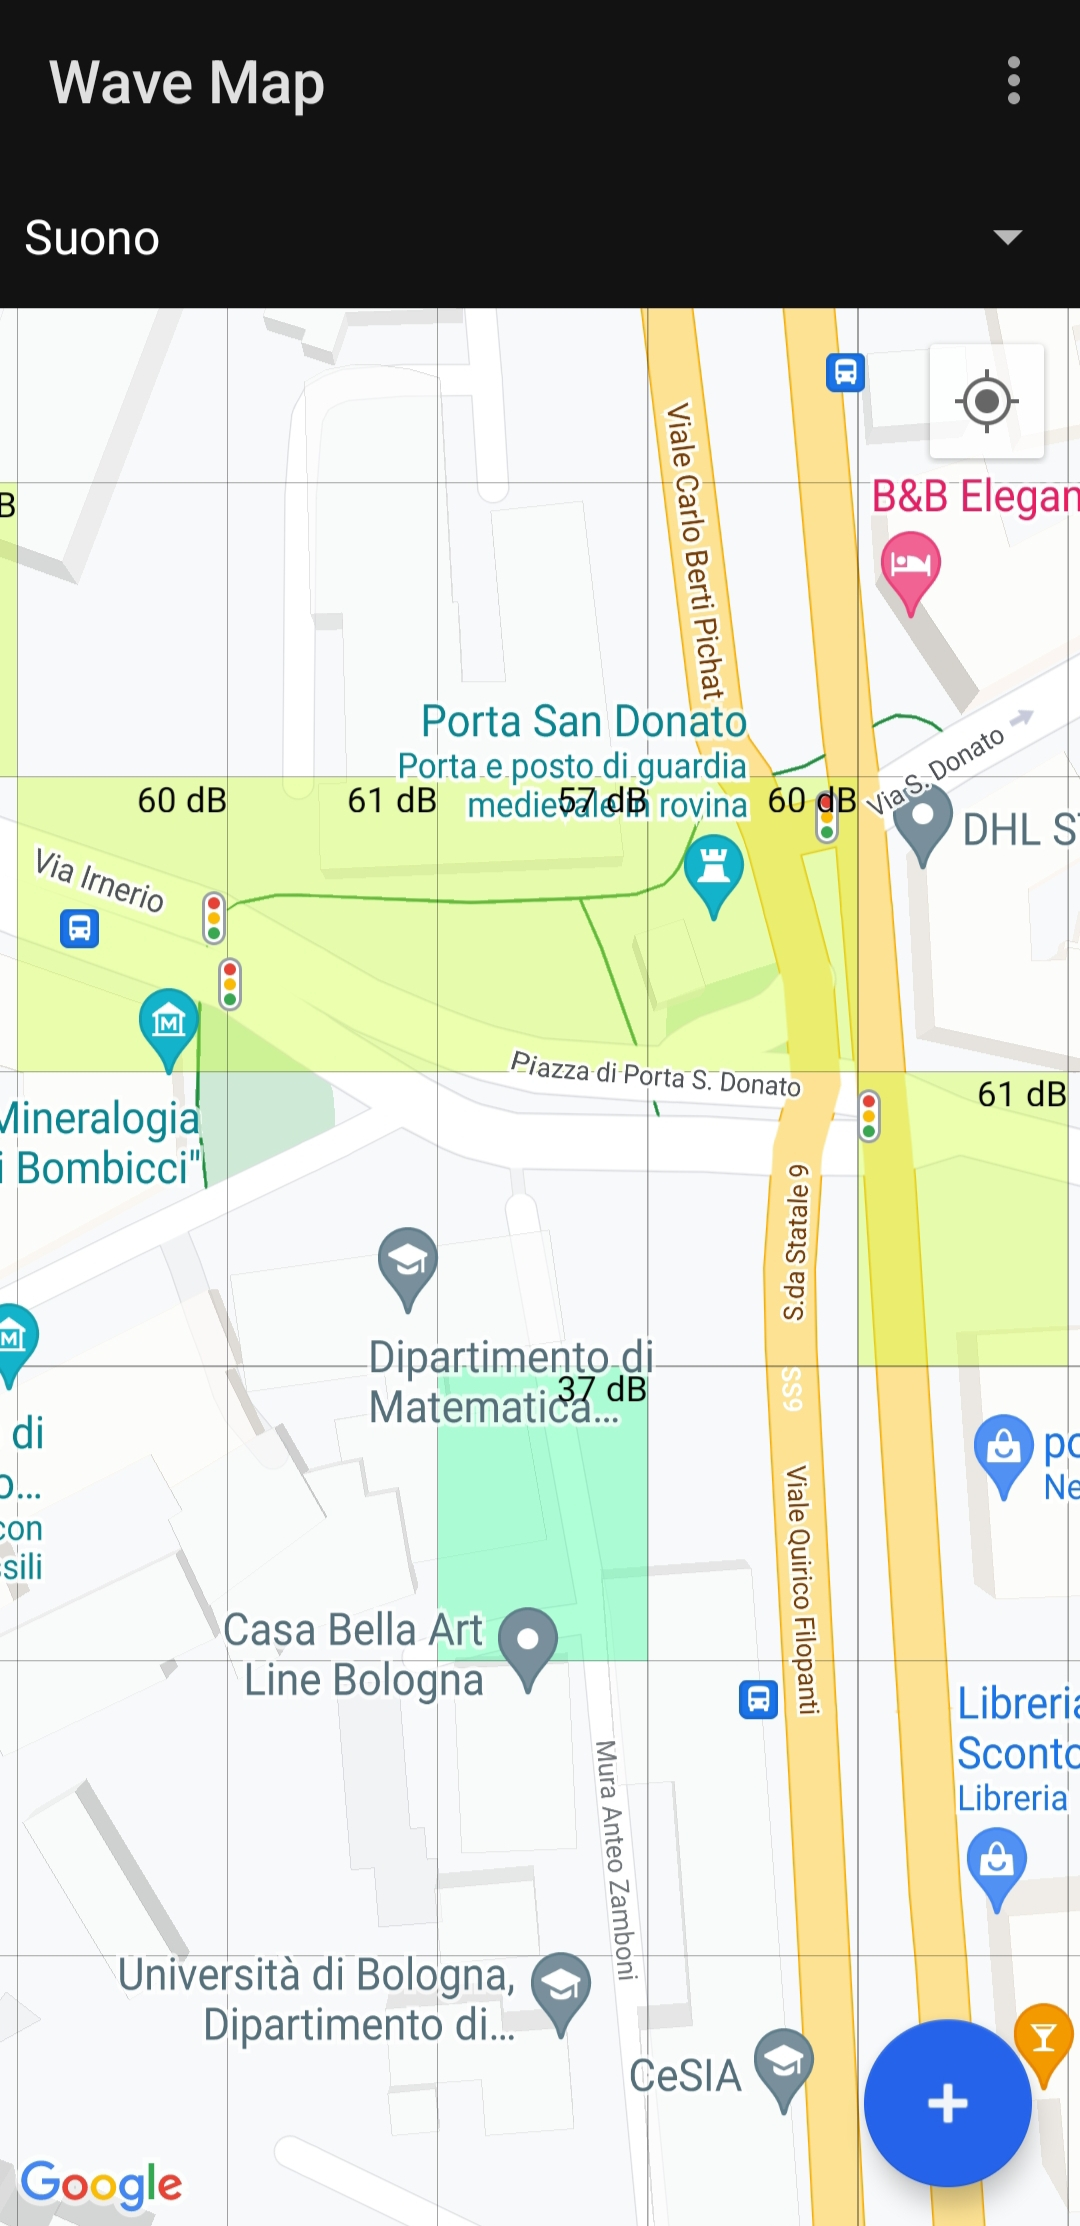
\includegraphics[width=\textwidth]{./img/overview/map_zoom1.jpg}
      \caption*{Suddivisione in 3 range}
    \end{minipage}
    \hspace*{1cm}
    \begin{minipage}[b]{0.25\textwidth}
      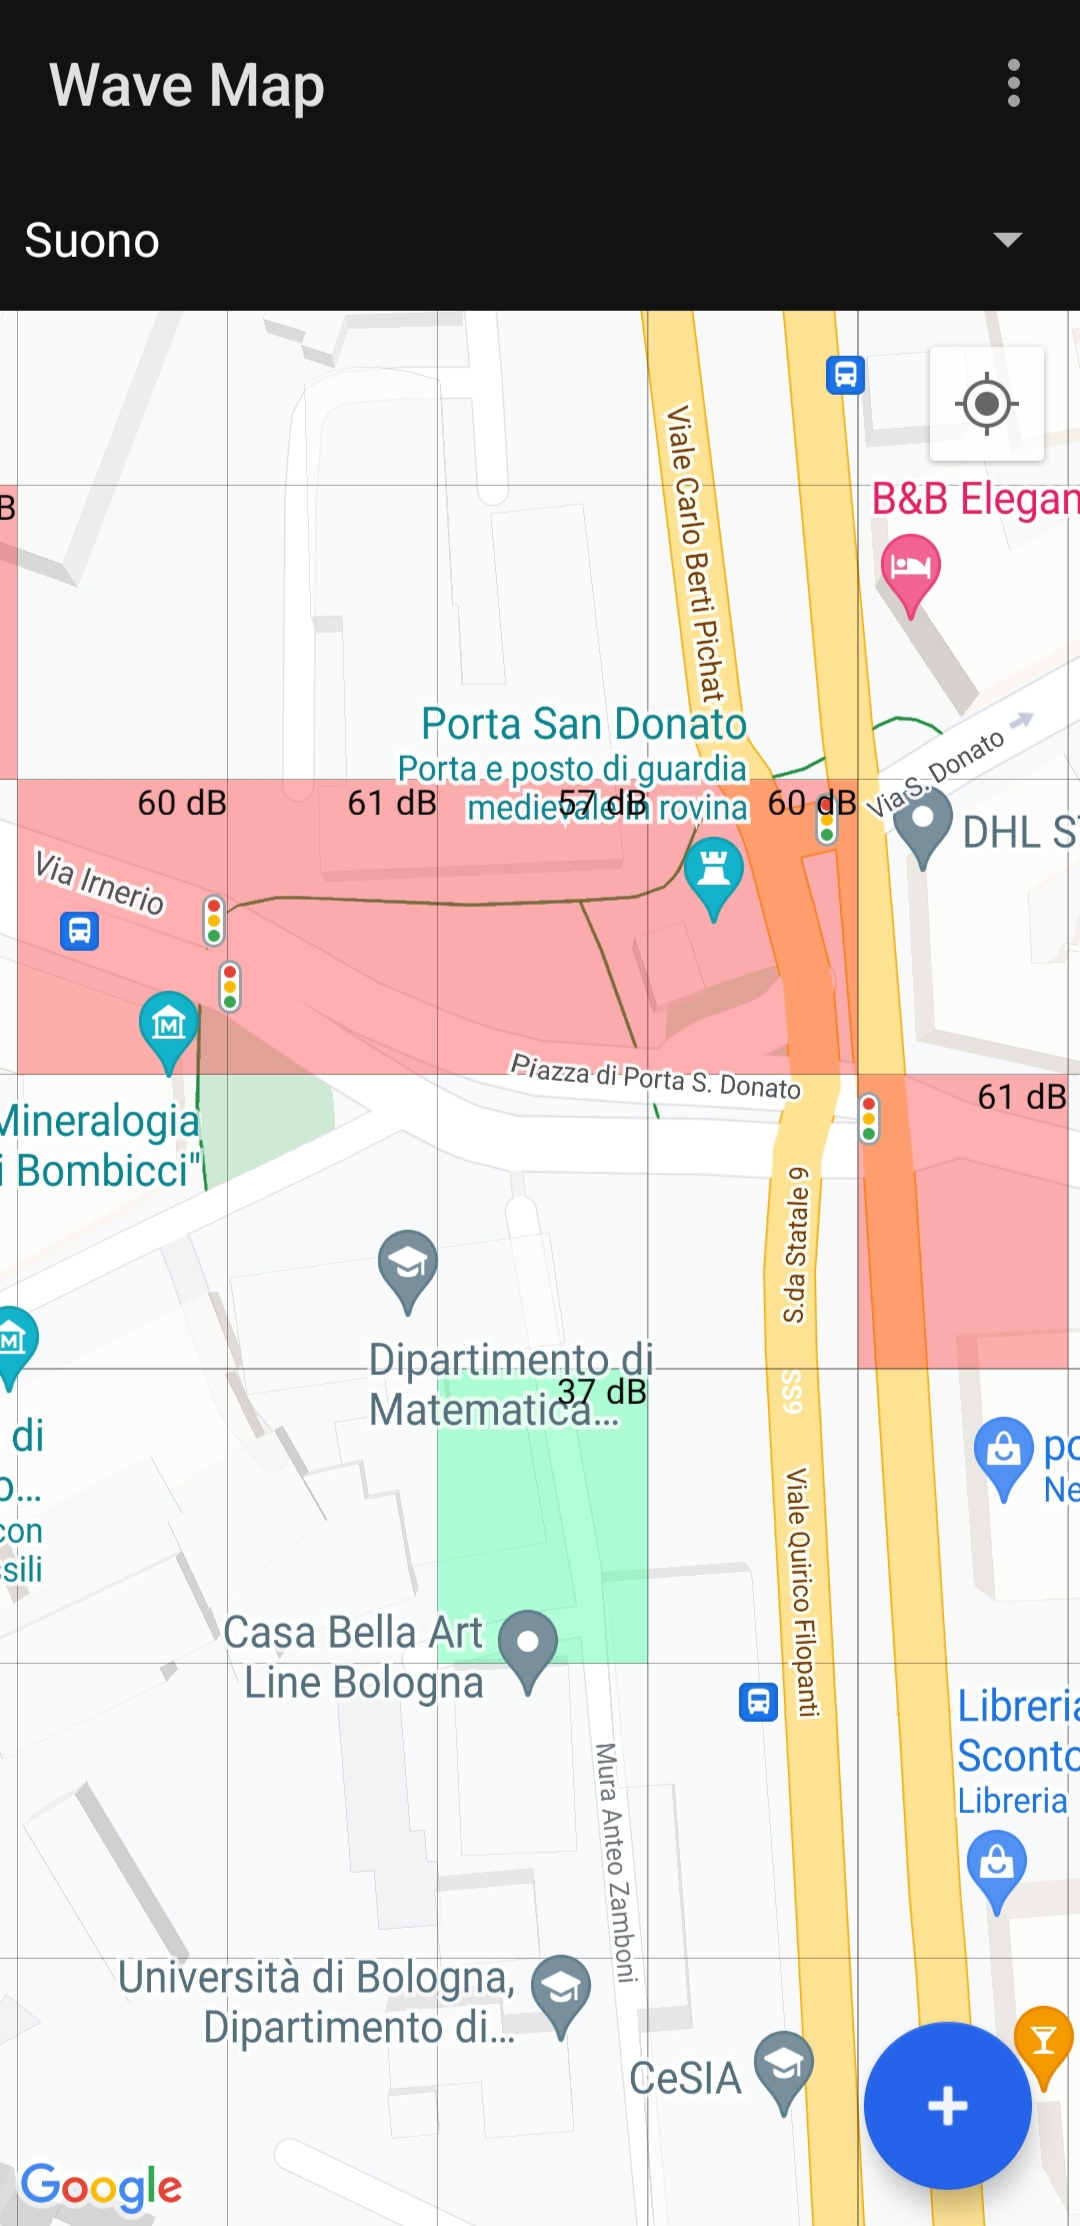
\includegraphics[width=\textwidth]{./img/overview/map_ranges.jpg}
      \caption*{Suddivisione in 2 range}
    \end{minipage}
    \caption{Range di qualità delle misurazioni calcolati algoritmicamente} \label{fig:overview_ranges}
\end{figure}

\begin{figure}[H]
    \centering
    \begin{minipage}[b]{0.25\textwidth}
      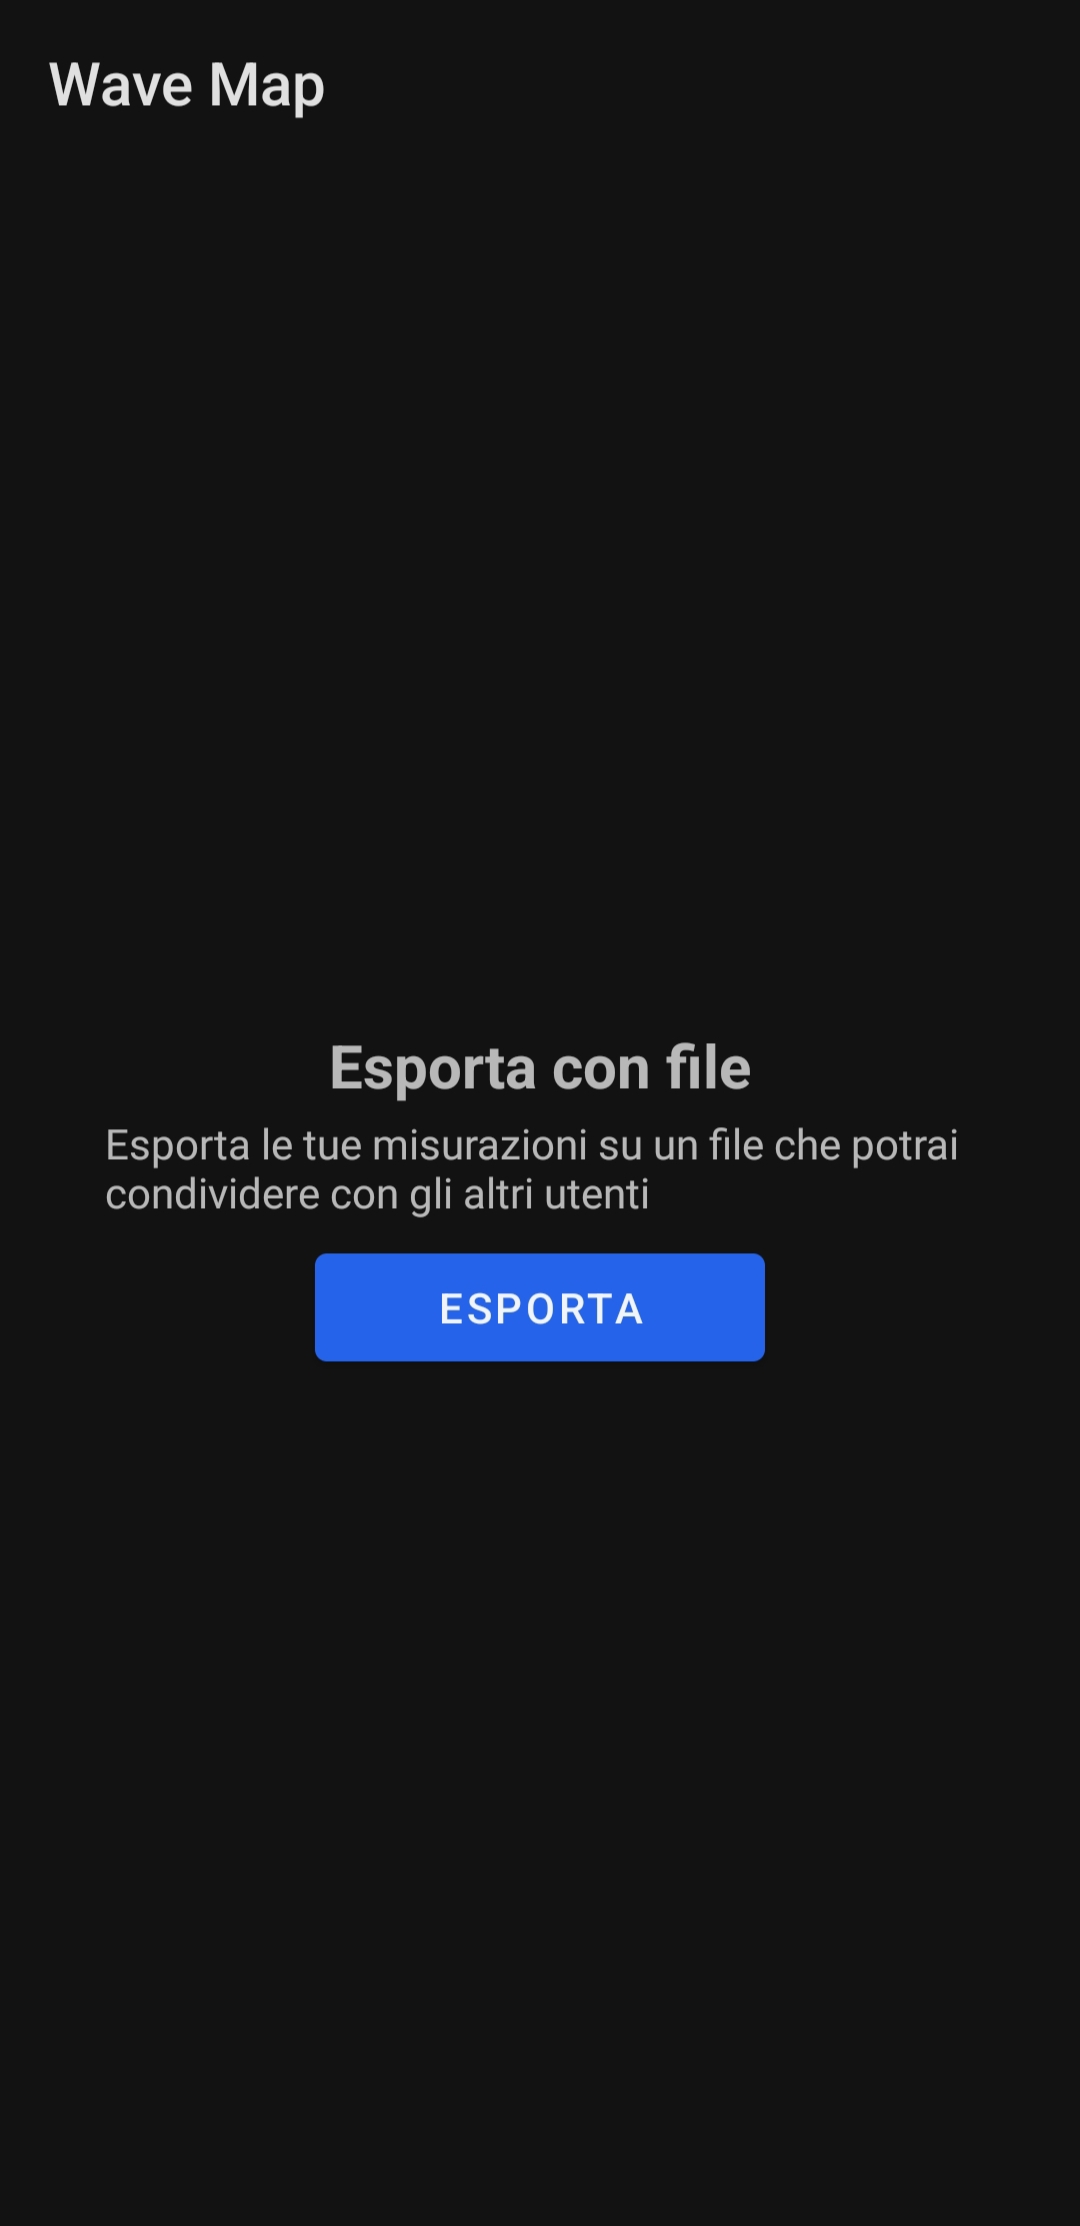
\includegraphics[width=\textwidth]{./img/overview/export1.jpg}
    \end{minipage}
    \begin{minipage}[b]{0.25\textwidth}
      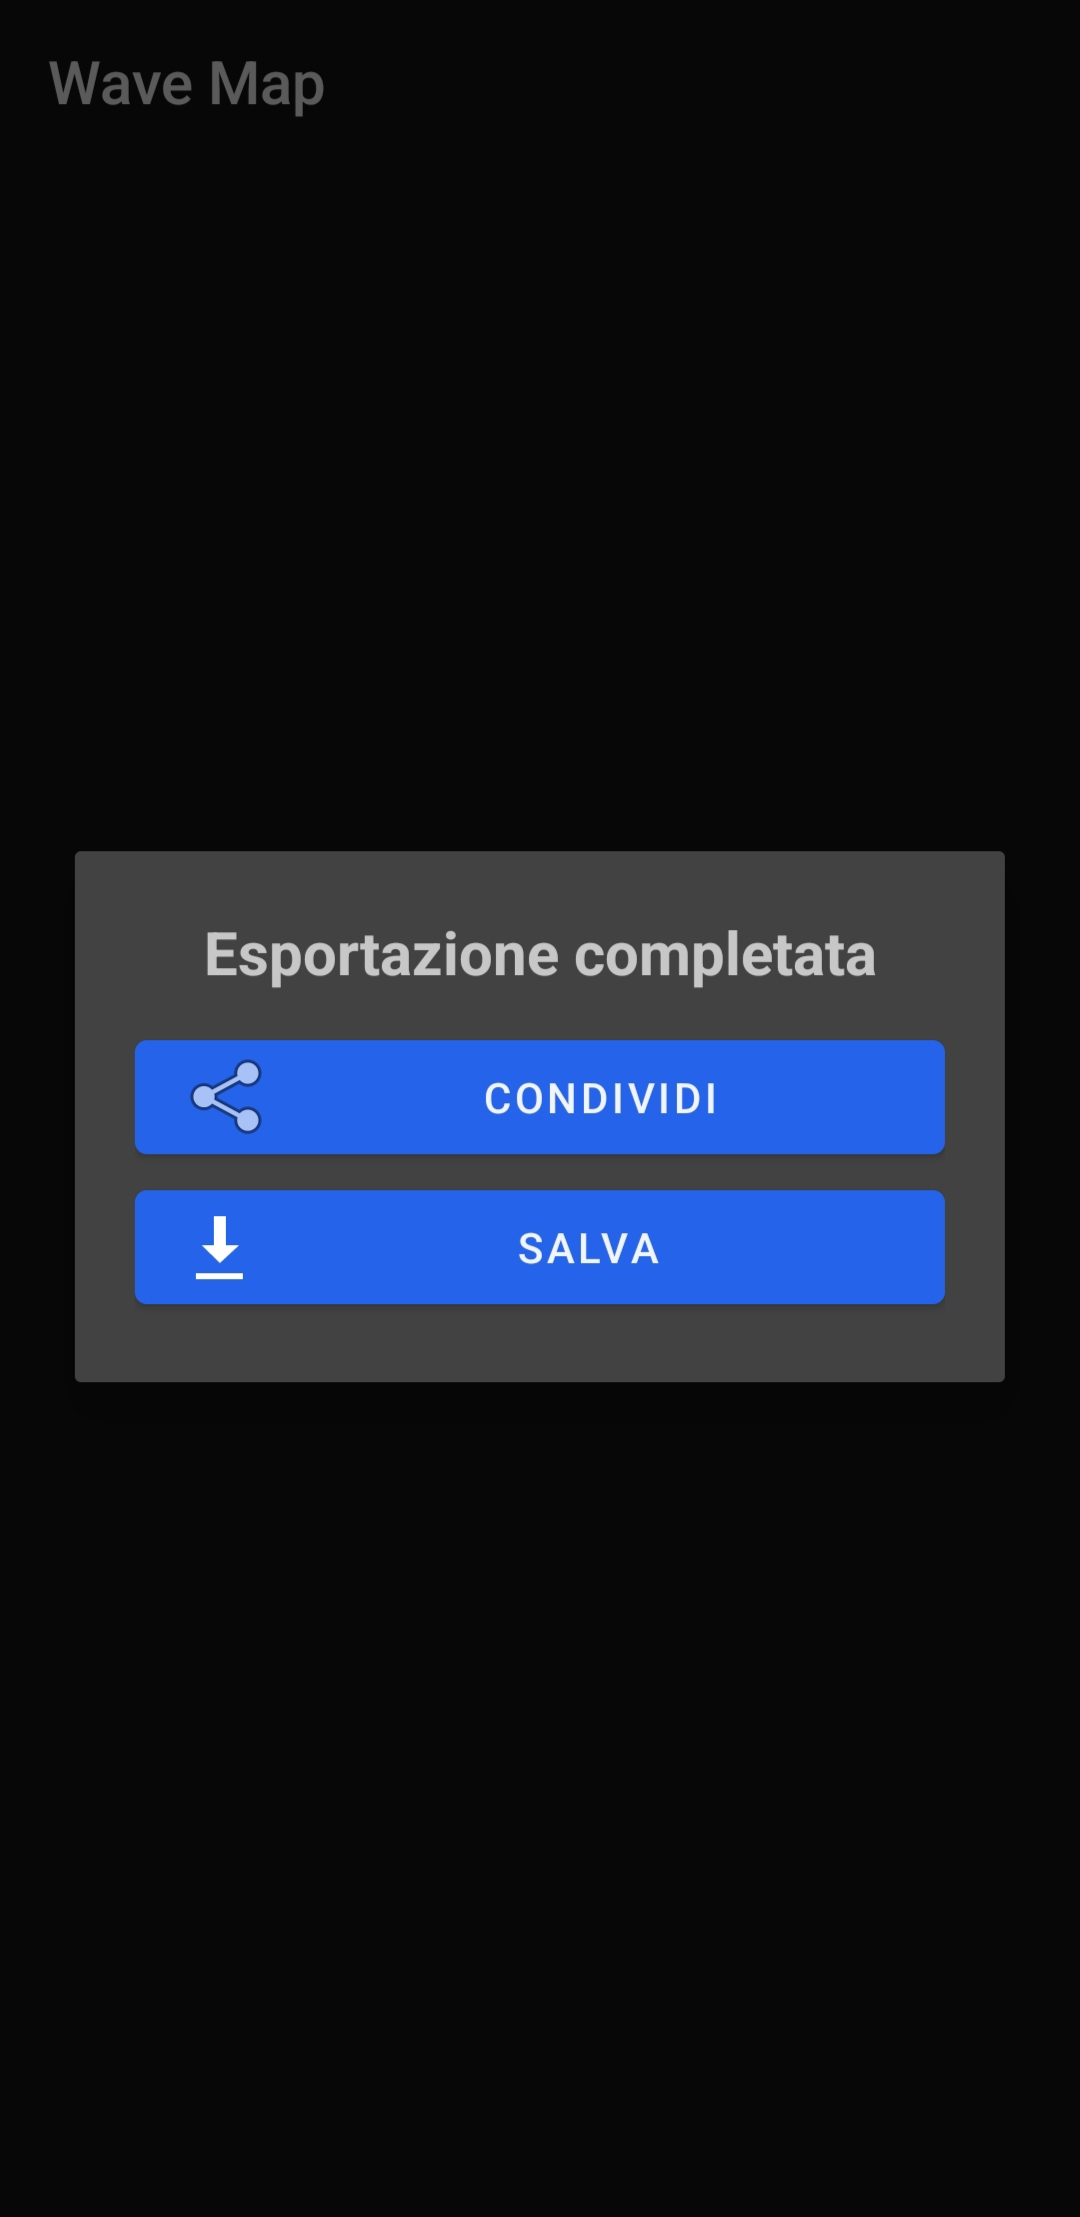
\includegraphics[width=\textwidth]{./img/overview/export2.jpg}
    \end{minipage}
    \hspace*{1cm}
    \begin{minipage}[b]{0.25\textwidth}
      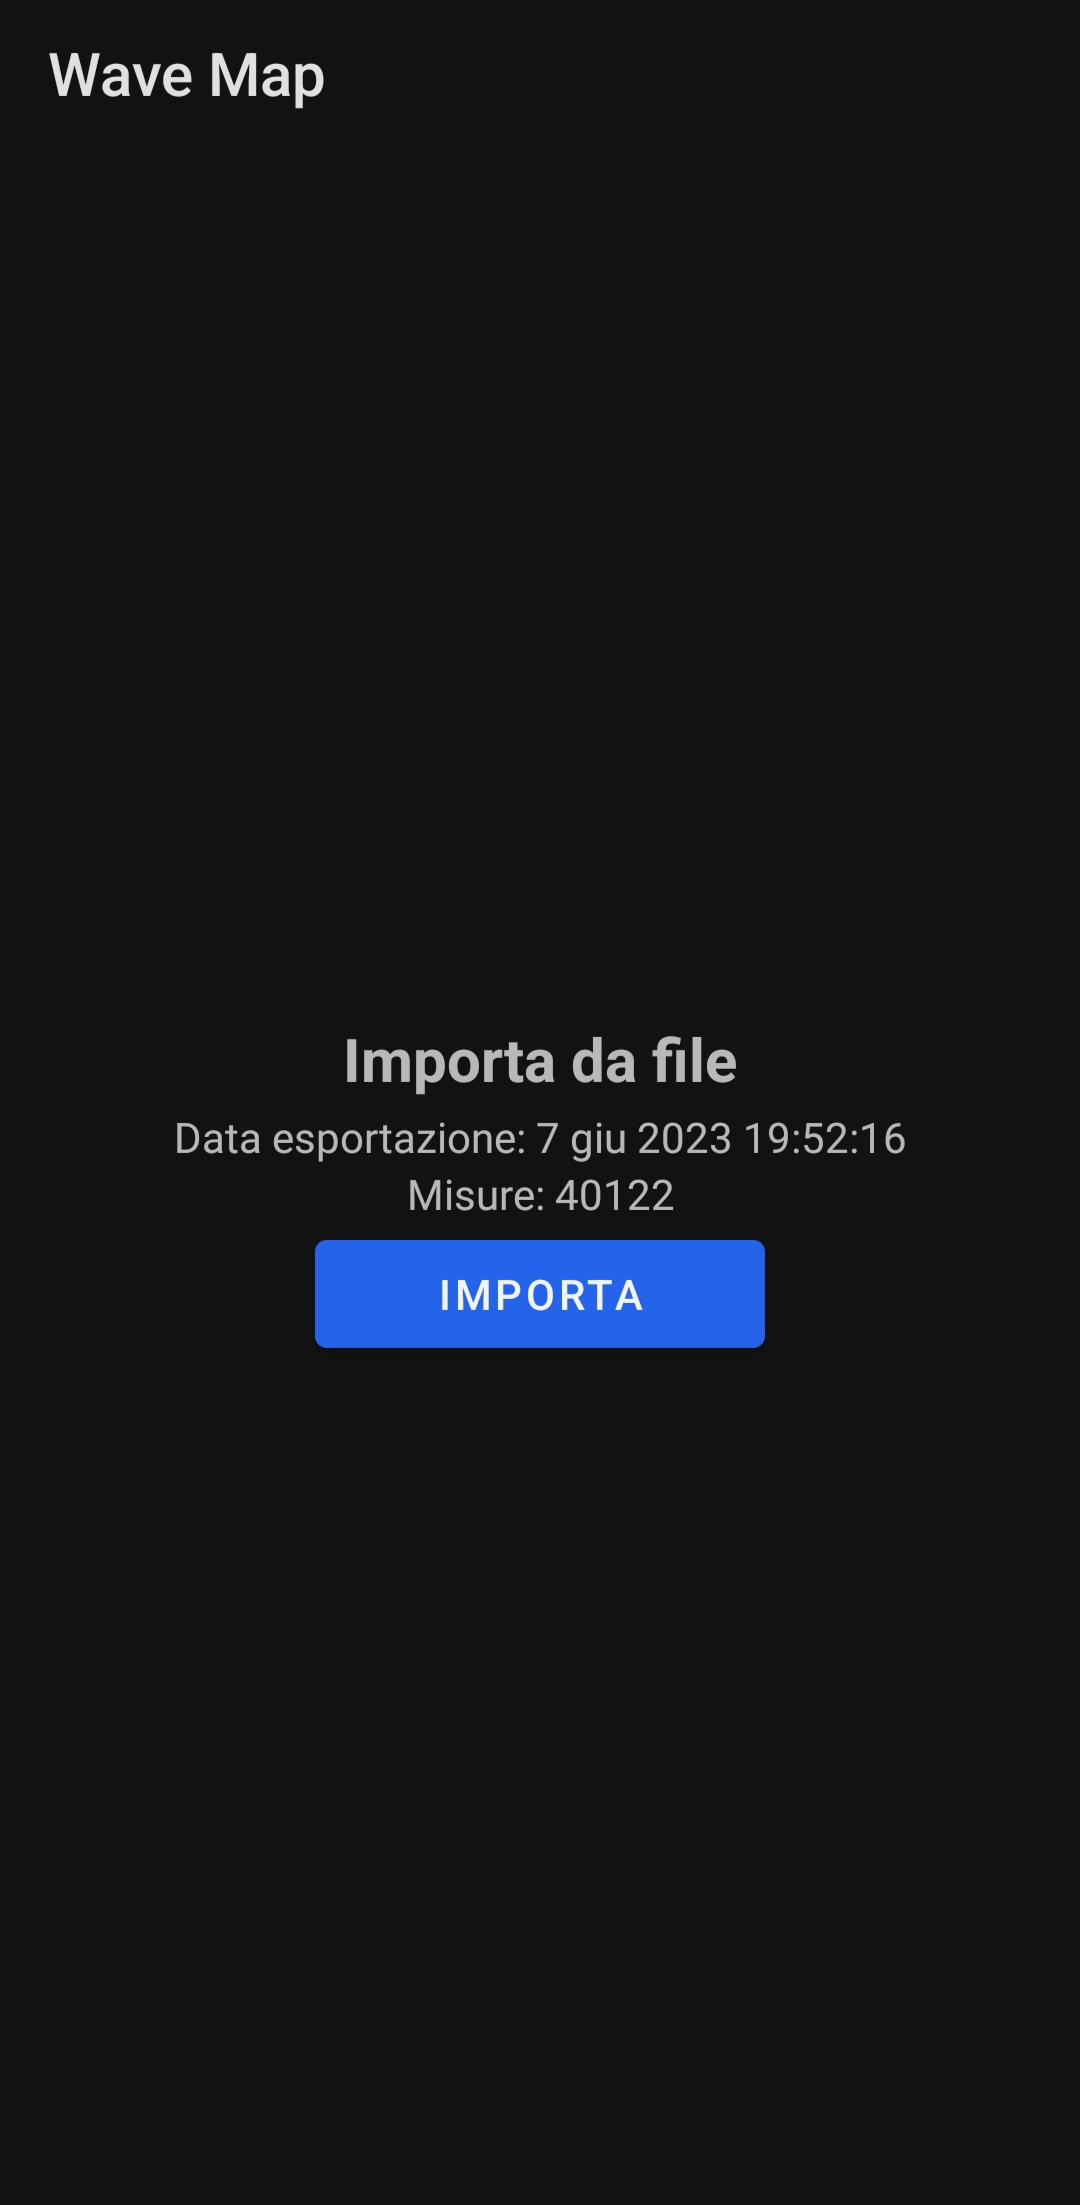
\includegraphics[width=\textwidth]{./img/overview/import.jpg}
    \end{minipage}
    \caption{Esportazione e importazione da file} \label{fig:overview_import_export}
\end{figure}

\begin{minipage}[b]{0.45\textwidth}
  \begin{figure}[H]
    \centering
    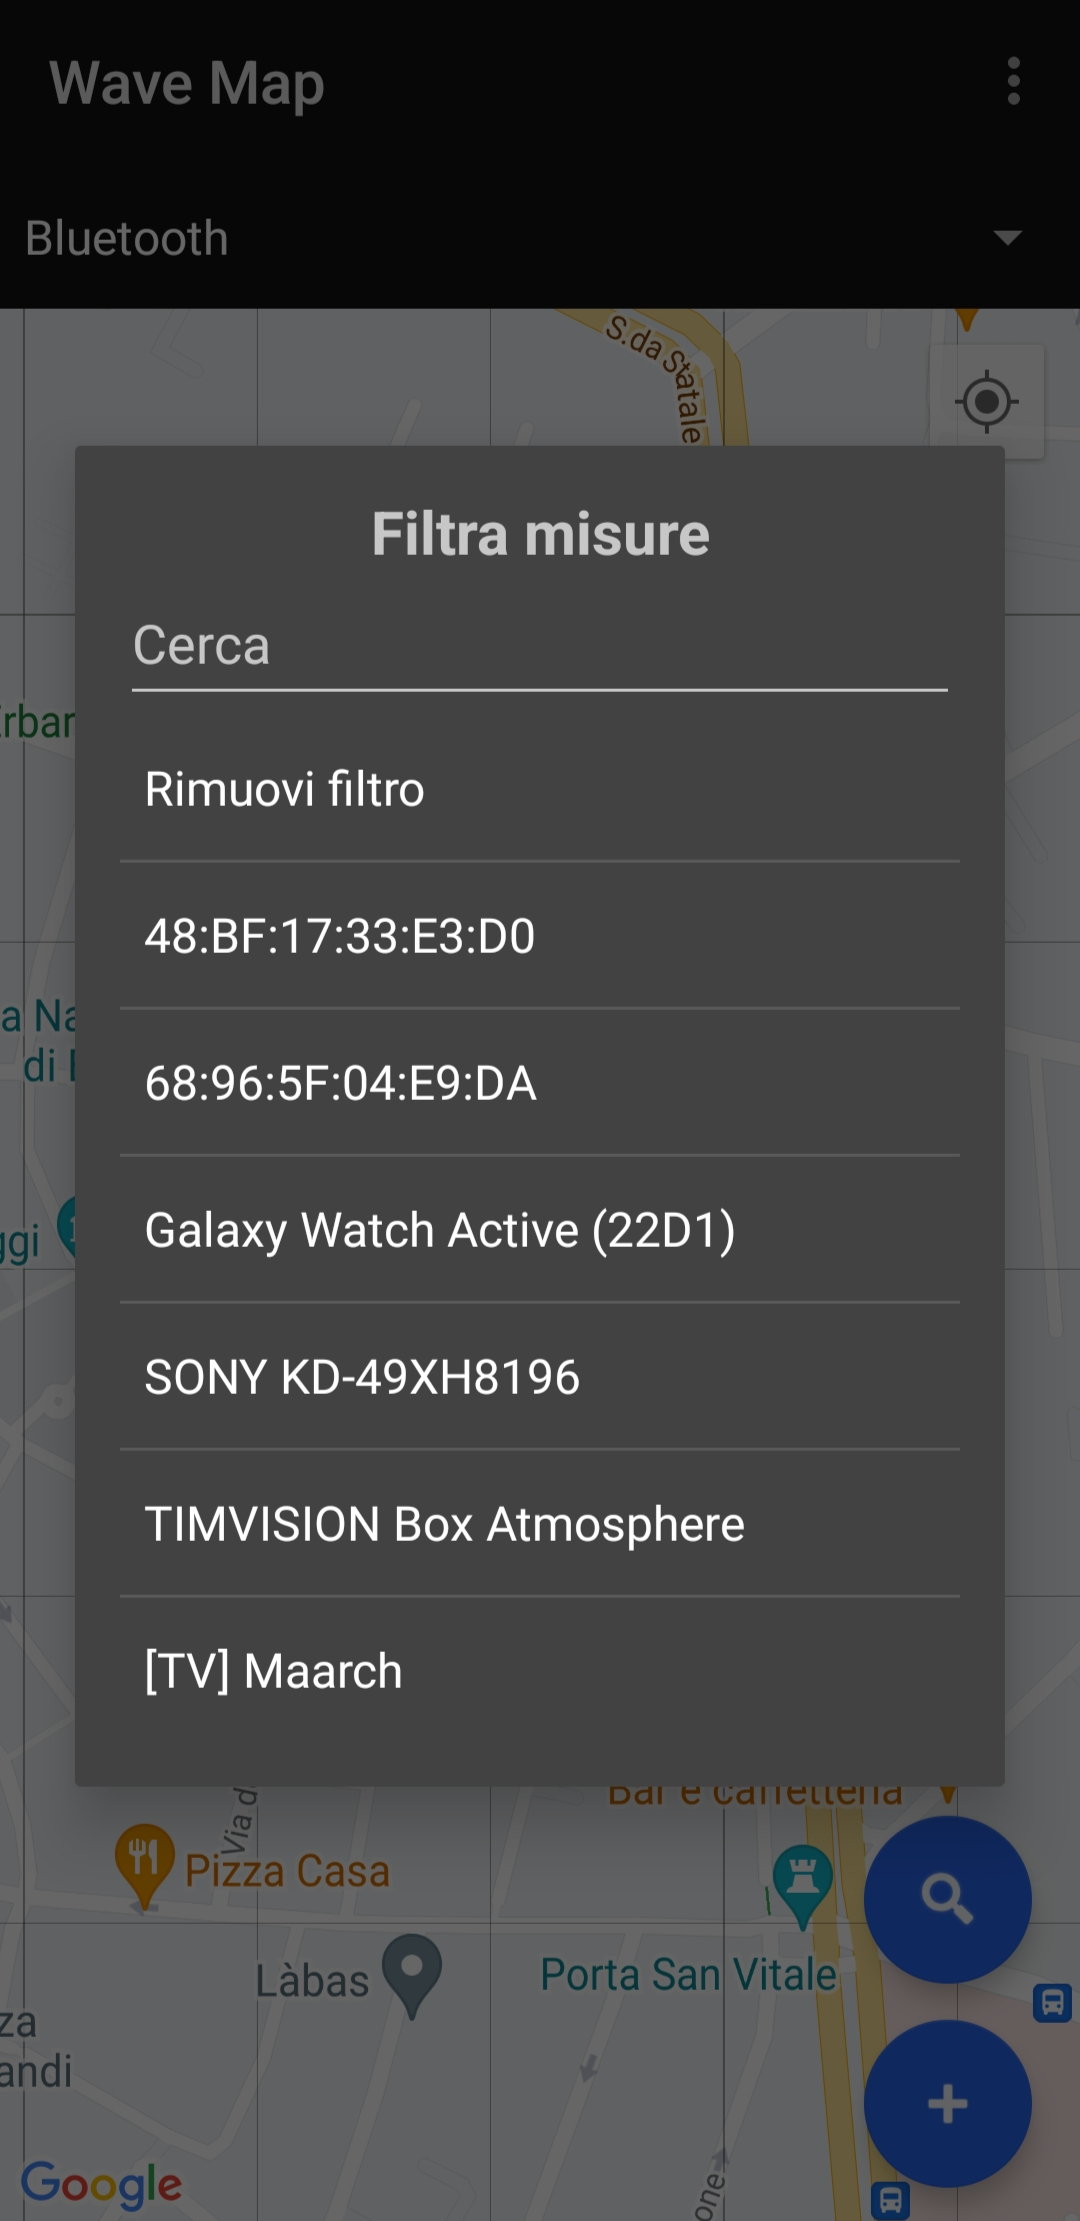
\includegraphics[width=0.50\textwidth]{./img/overview/query.jpg}
    \caption{Filtro di ricerca} \label{fig:query}
  \end{figure}
\end{minipage}
\hfill
\begin{minipage}[b]{0.45\textwidth}
  \begin{figure}[H]
    \centering
    \begin{minipage}[b]{0.35\textwidth}
      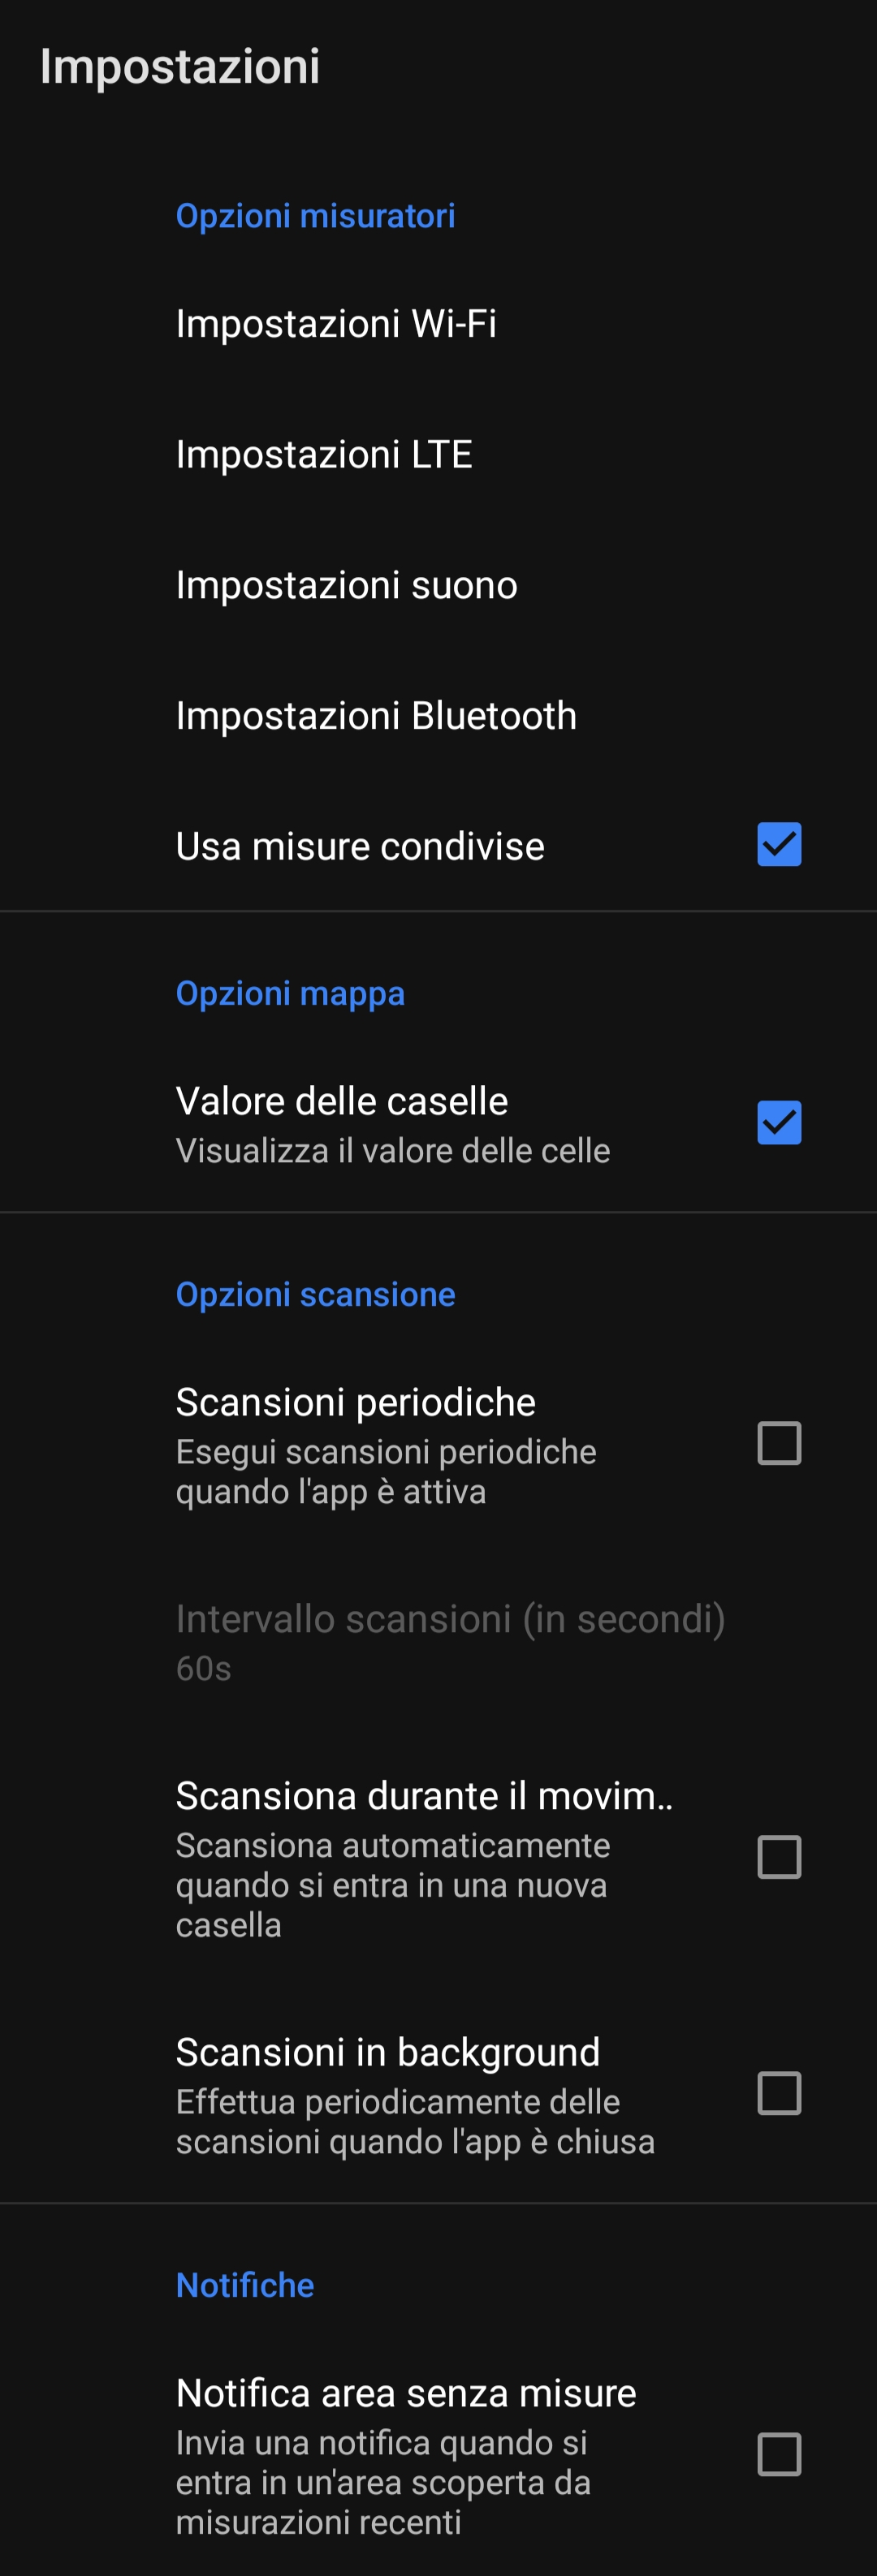
\includegraphics[width=\textwidth]{./img/overview/settings1.jpg}
    \end{minipage}
    \hspace*{1cm}
    \begin{minipage}[b]{0.45\textwidth}
      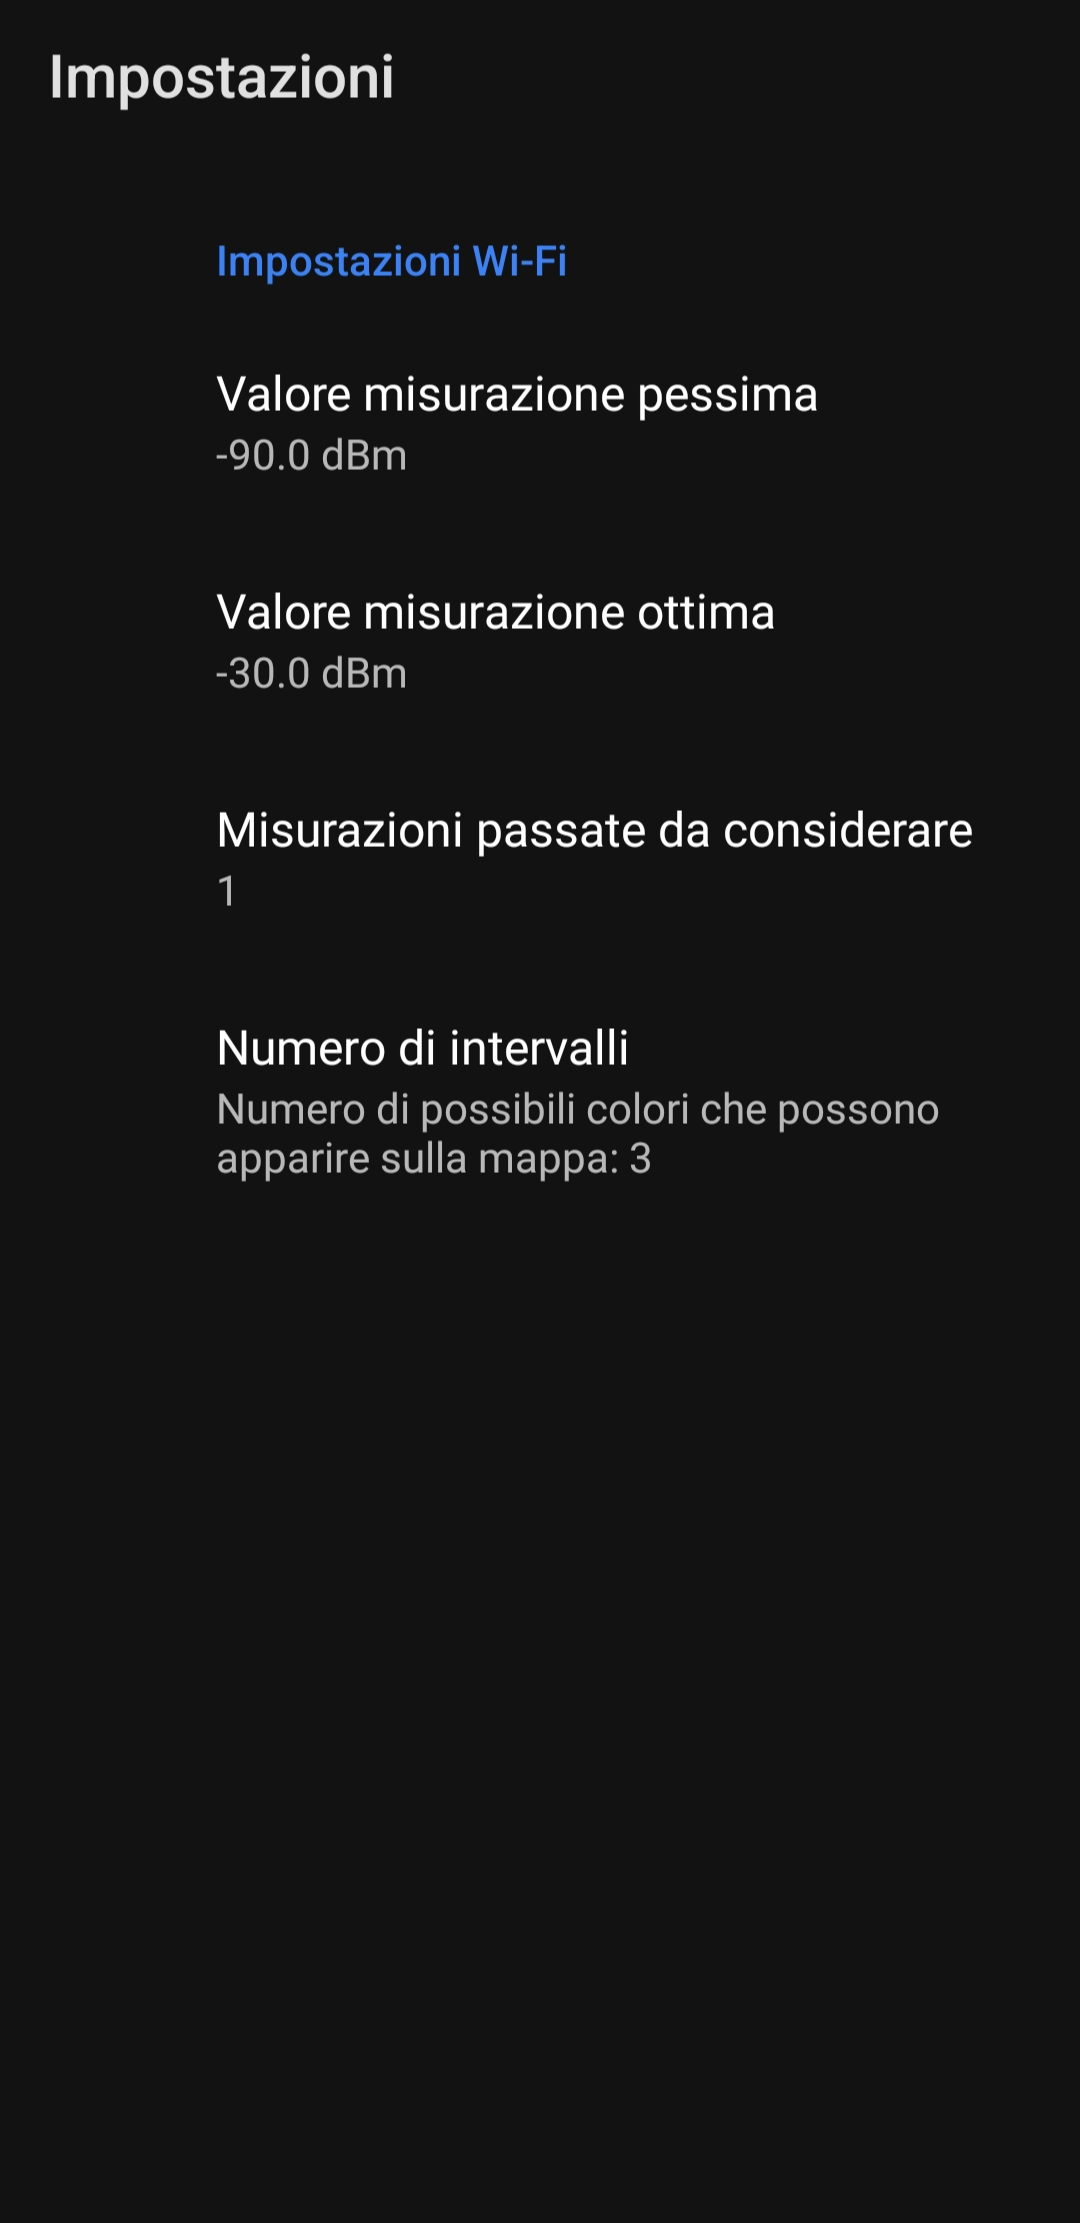
\includegraphics[width=\textwidth]{./img/overview/settings2.jpg}
    \end{minipage}
    \caption{Impostazioni} \label{fig:settings}
  \end{figure}
\end{minipage}


\section{Scelte progettuali}

\subsection{Informazioni generali}
Il progetto è stato sviluppato come applicazione nativa utilizzando Kotlin. 
Come pattern architetturale è stato principalmente utilizzato l'approccio Model-View-ViewModel, mentre per l'interfacciamento con il database locale è stata utilizzata la libreria \texttt{Room}.

Le operazioni asincrone sono state principalmente implementate tramite le \texttt{coroutine} e per favorire un codice più "lineare", quando possibile, sono state trasformate le funzioni con callback in funzioni \texttt{suspend} utilizzando come wrapper \texttt{suspendCoroutine}.

\subsubsection{Organizzazione dei package}
L'organizzazione dei package è la seguente:
\begin{table}[H]
  \centering
  \begin{tabular}{ | m{8em} | m{10cm} | } 
    \hline
    \texttt{db} & Classi che implementano la struttura e le operazioni sulle tabelle del database. \\ 
    \hline
    \texttt{dialogs} & Classi per istanziare i dialog utilizzati nell'applicazione. \\ 
    \hline
    \texttt{notifications} & Classi per istanziare le notifiche utilizzate nell'applicazione. \\ 
    \hline
    \texttt{measures} & Classi che implementano le operazioni per effettuare le misurazioni. \\ 
    \hline
    \texttt{services} & Classi che implementano i servizi in background. \\ 
    \hline
    \texttt{ui} & \texttt{Activity}, \texttt{Fragment} e \texttt{ViewModel} dell'applicazione. \\ 
    \hline
    \texttt{utilities} & Metodi e variabili di utilità generale. \\ 
    \hline
  \end{tabular}
  \caption{Organizzazione package}\label{table:packages}
\end{table}

\subsection{Raccolta dei dati}

\subsubsection{Struttura e memorizzazione delle misurazioni}
Una misurazione è descritta dall'interfaccia \texttt{WaveMeasure} e contiene il valore della misurazione, un timestamp, la posizione e un flag per indicare se si tratta di una misurazione propria o ottenuta tramite condivisione. 
In aggiunta, è presente un campo per informazioni aggiuntive utile per distinguere alcune tipologie di misurazioni (es. per Wi-Fi e Bluetooth viene salvato il BSSID).

L'interfaccia \texttt{WaveMeasure} viene quindi utilizzata per implementare la classe \texttt{MeasureTable} che descrive la tabella del database dedicata alla memorizzazione delle misurazioni. 
Tutte le misurazioni sono salvate nella stessa tabella e sono differenziate da un campo (\texttt{type}) aggiunto in fase di salvataggio nel database.
Inoltre, ciascuna misura è identificata univocamente da un UUID, utile anche per differenziare le misurazioni provenienti da altri utenti.

In aggiunta, una seconda tabella descritta dalla classe \texttt{BSSIDTable} contiene la mappatura da BSSID a SSID.


\subsubsection{Sampler}
Per la raccolta dei dati è stato introdotto il concetto di \textit{sampler} per gestire in maniera modulare le misurazioni.
Nello specifico, un \textit{sampler} è descritto dalla classe astratta \texttt{WaveSampler} e richiede l'implementazione dei seguenti metodi:
\begin{itemize}
    \item \texttt{sample} per prendere una nuova misurazione.
    \item \texttt{store} per il salvataggio dei dati nel database.
    \item \texttt{retrieve} per la ricerca dei dati note le coordinate dei vertici di una cella della mappa.
\end{itemize}
Inoltre, sono esposte le seguenti funzioni ausiliarie:
\begin{itemize}
    \item \texttt{average} richiama \texttt{retrieve} e restituisce la media dei valori.
    \item \texttt{sampleAndStore} richiama in sequenza \texttt{sample} e \texttt{store}.
\end{itemize}
Per maggiore flessibilità, le misure vengono sempre intese come liste di \texttt{WaveMeasure}. Ciò permette di gestire misurazioni che per loro natura non generano un'unica misurazione (es. Wi-Fi e Bluetooth).

A partire da \texttt{WaveSampler} sono quindi implementati i \textit{sampler} per:
\begin{itemize}
  \item Wi-Fi (\texttt{WiFiSampler}): 
    \begin{itemize}[topsep=0em]
      \item Ottiene la potenza della rete al quale il dispositivo è attualmente connesso tramite il servizio di sistema \texttt{ConnectivityManager}. Per versioni inferiori alla API 29, viene invece utilizzato il \texttt{WifiManager}.
      \item Misura la potenza delle reti circostanti registrando un \texttt{BroadcastReceiver} con filtro \texttt{WifiManager.SCAN\_RESULTS\_AVAILABLE\_ACTION} e richiedendo una scansione completa attraverso il \texttt{WifiManager}.
    \end{itemize}
  \item Bluetooth (\texttt{BluetoothSampler}):
    \begin{itemize}[topsep=0em]
      \item Misura la potenza dei dispositivi accoppiati mediante il \texttt{BluetoothManager}.
      \item Misura la potenza dei dispositivi circostanti registrando un \texttt{BroadcastReceiver} con filtro \texttt{BluetoothDevice.ACTION\_FOUND} e richiedendo al \texttt{BluetoothManager} una scansione completa.
    \end{itemize}
  \item LTE (\texttt{LTESampler}): ottiene la potenza del segnale LTE tramite il \texttt{TelephonyManager}.
  \item Suono (\texttt{NoiseSampler}): viene fatta la media di una serie di campionature effettuate utilizzando un \texttt{MediaRecorder}.
\end{itemize}

\subsection{Mappa}
Per la mappa è stato utilizzato \gmaps{} e l'implementazione è contenuta in \texttt{WaveHeatMapFragment}.

Il fragment \texttt{WaveHeatMapFragment} gestisce la generazione delle celle e utilizza un \texttt{MeasureViewModel} (descritto in \cref{sec:MeasureViewModel}) per interfacciarsi con i dati delle misurazioni.

Inoltre, espone all'esterno due metodi e un \texttt{LiveData}: i metodi permettono di cambiare tipologia di misurazione e rigenerare la mappa attualmente visibile, mentre il \texttt{LiveData} notifica gli spostamenti di cella del dispositivo.


\subsubsection{Generazione cella}
Una cella della mappa rappresenta la misurazione di un'area quadrata\footnote{Esclusa la zona equatoriale, le celle appariranno rettangolari} e la dimensione di quest'ultima scala automaticamente in base al livello dello zoom.

Una cella è descritta dalle coordinate del vertice superiore sinistro (nord-ovest) e a partire da questa vengono calcolate le coordinate degli altri convertendo la dimensione della cella (in metri) in un offset da applicare a latitudine e longitudine.
Per questioni estetiche, gli offset sono approssimati in modo tale che tutte le righe siano allineate verticalmente (\cref{fig:tile_offset}).
\begin{figure}[H]
    \centering
    \begin{minipage}[b]{0.45\textwidth}
      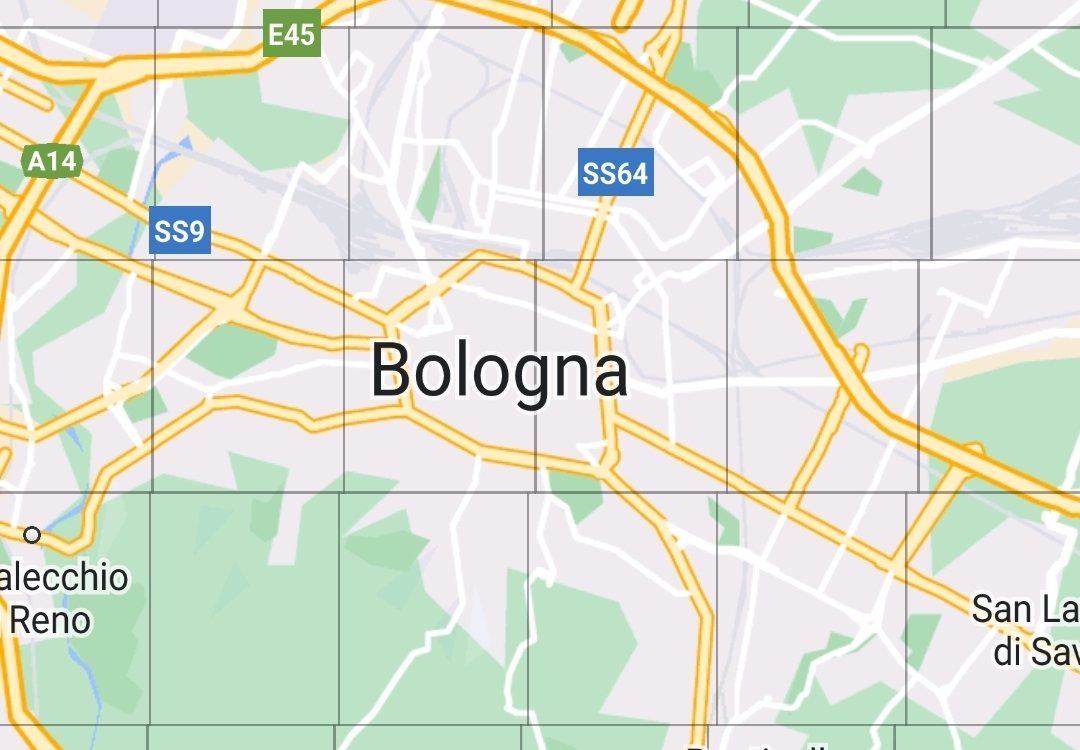
\includegraphics[width=\textwidth]{./img/tile_no_approx.jpg}
    \end{minipage}
    \hfill
    \begin{minipage}[b]{0.45\textwidth}
      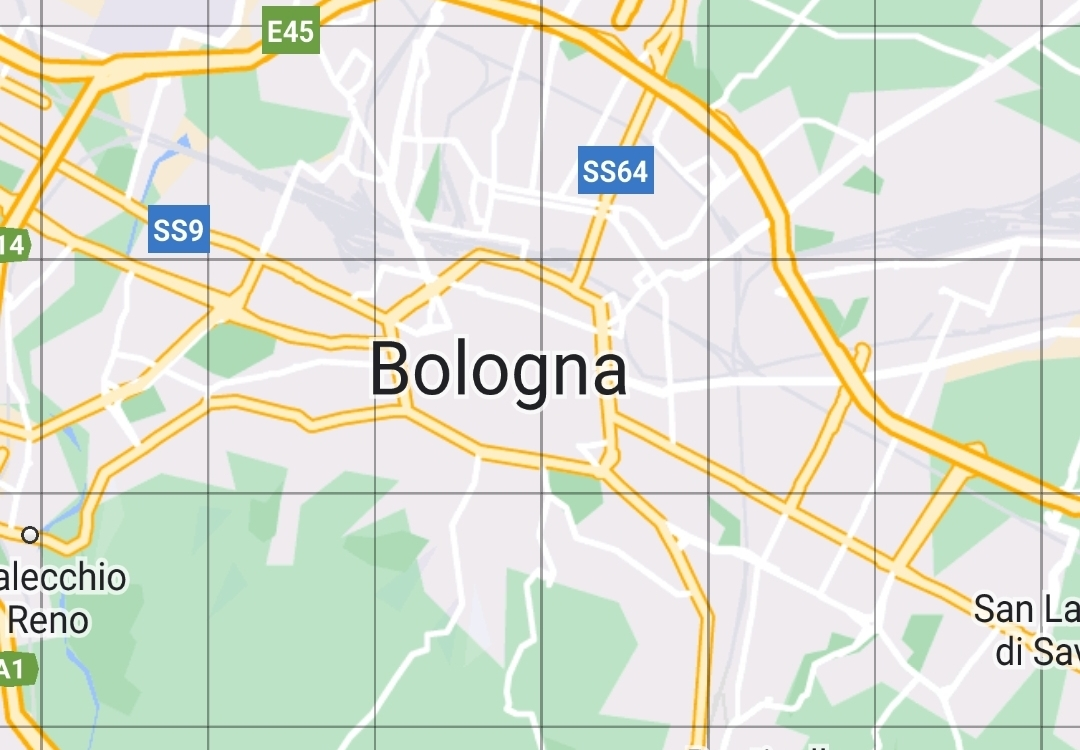
\includegraphics[width=\textwidth]{./img/tile_approx.jpg}
    \end{minipage}
    \caption{Offset calcolati in maniera precisa (sinistra) e approssimata (destra)} \label{fig:tile_offset}
\end{figure}

Il colore di una cella è determinato dal valore e dal tipo di misurazione, e viene impostato in formato HSV modificando il valore della tinta (hue).
Per ciascuna tipologia di misurazione sono specificati gli estremi del range di qualità e il numero di intervalli in cui suddividerlo.
La tinta è quindi determinata collocando il valore della misurazione in uno dei sotto-intervalli del range e selezionando come valore finale l'estremo inferiore (\cref{alg:hue}).

\begin{algorithm}[H]
  \caption{Tinta di una cella}\label{alg:hue}
  \SetAlgoLined
  \SetKwProg{Fn}{fun}{}{end}
  \Fn{\textup{\texttt{{getHue(measure, measure\_range=[$a$, $b$], hue\_range=[$0$, $150$], n\_ranges)}}}}{
    $\texttt{hue} \gets \text{\texttt{measure} scalata da \texttt{measure\_range} a \texttt{hue\_range}}$\\
    $\texttt{hue} \gets \text{\texttt{hue} discretizzata in \texttt{hue\_range} suddiviso in \texttt{n\_ranges} valori}$\\
    return \texttt{hue}
  }
\end{algorithm}

Infine, per ogni cella è presente un'etichetta contenente il valore della misurazione. Poiché \gmaps{} non permette di inserire esplicitamente del testo nella mappa, l'implementazione prevede di generare l'etichetta come un'immagine che viene poi impostata come icona di un marker. Inoltre, in caso di necessità, la dimensione del testo viene scalata per far in modo che rientri nei limiti della cella.


\subsubsection{Generazione griglia}
La griglia è composta da celle generate relativamente ad una posizione di riferimento. In particolare, in fase di inizializzazione viene designata come cella di riferimento quella che pone la posizione dell'utente al centro e in base a questa è possibile determinare la posizione di tutte le altre celle della mappa. 

Nello specifico, date le coordinate nord-ovest della cella di riferimento $(\texttt{center\_top\_left}_{\texttt{lat}}, \texttt{center\_top\_left}_{\texttt{lon}})$ e delle coordinate qualsiasi $(\texttt{pos}_{\texttt{lat}}, \texttt{pos}_{\texttt{lon}})$, per determinare la cella che la contiene si calcola il numero di celle da saltare rispetto a quella di riferimento: 
\begin{equation*}
    \texttt{to\_skip\_tiles}_\texttt{lat} =
        \lceil \frac{\texttt{pos}_{\texttt{lat}} - \texttt{center\_top\_left}_{\texttt{lat}}}{\texttt{latitudeOffset(tile\_length\_meters)}} \rceil
\end{equation*}
\begin{equation*}
    \texttt{to\_skip\_tiles}_\texttt{lon} =
        \lfloor \frac{\texttt{pos}_{\texttt{lon}} - \texttt{center\_top\_left}_{\texttt{lon}}}{\texttt{longitudeOffset(tile\_length\_meters)}} \rfloor
\end{equation*}
Le coordinate del vertice superiore sinistro della cella che contiene $(\texttt{pos}_{\texttt{lat}}, \texttt{pos}_{\texttt{lon}})$ sono quindi:
\begin{equation*}
    \texttt{tile}_\texttt{lat} = \texttt{center\_top\_left}_{\texttt{lat}} + (\texttt{to\_skip\_tiles}_\texttt{lat} \cdot \texttt{latitudeOffset(tile\_length\_meters)})
\end{equation*}
\begin{equation*}
    \texttt{tile}_\texttt{lon} = \texttt{center\_top\_left}_{\texttt{lon}} + (\texttt{to\_skip\_tiles}_\texttt{lon} \cdot \texttt{longitudeOffset(tile\_length\_meters)})
\end{equation*}

Con questo approccio, ogni volta che viene spostata la visuale della mappa, la griglia viene generata iterando a partire dalle coordinate dell'angolo nord-ovest visibile dello schermo, fino a raggiungere l'angolo sud-est. 

In aggiunta, per maggiore efficienza, si tiene traccia delle celle generate in modo da evitare di dover ridisegnare l'intera area visibile ad ogni movimento della mappa. Questo meccanismo viene resettato quando viene cambiato il livello di zoom, in quanto tutte le celle già presenti diventano obsolete e vengono necessariamente cancellate.
\subsection{App principale}
% Il punto di entrata del programma è l'activity \texttt{MainActivity} che contiene la mappa e i comandi per effettuare le misurazioni.

\subsubsection{ViewModel dei \textit{sampler}} \label{sec:MeasureViewModel}
Per ciascun \textit{sampler} è stato definito un ViewModel dedicato contenente le operazioni e le informazioni per ciascun tipo di misurazione.
In particolare, è stata definita una gerarchia di ViewModel come rappresentato in \cref{fig:viewmodel_hierarchy}.

\begin{figure}[H]
  \centering
  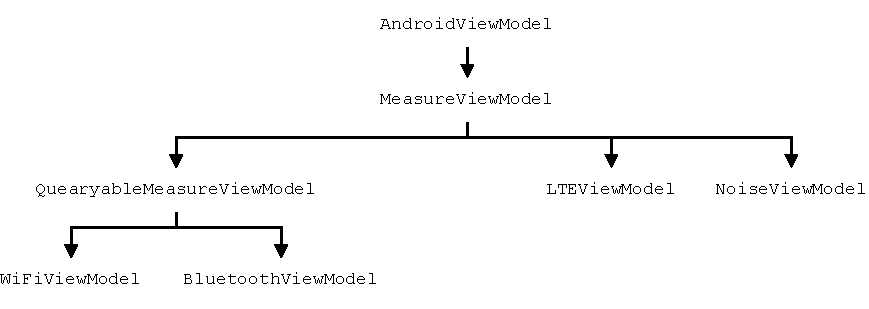
\includegraphics[width=\textwidth]{./img/viewmodel.pdf}
  \caption{Gerarchia dei ViewModel} \label{fig:viewmodel_hierarchy}
\end{figure}

La gerarchia ha come radice \texttt{AndroidViewModel} in quanto fornisce il \texttt{Context} dell'applicazione necessario per i \textit{sampler}.

La classe astratta \texttt{MeasureViewModel} fornisce tutte le informazioni utili per una tipologia di misurazione. Specificamente, contiene l'istanza del \texttt{WaveSampler} e i parametri quali: il range di qualità, il numero di intervalli, il numero di misure passate da considerare e un flag per indicare se caricare anche le misure condivise.
Vengono inoltre esposti i metodi per effettuare una nuova misurazione, ottenere la media delle misurazioni di una casella e caricare le impostazioni specifiche per il tipo di misura.
Da \texttt{MeasureViewModel} sono implementati \texttt{LTEViewModel} e \texttt{NoiseViewModel}.

\texttt{MeasureViewModel} viene poi estesa in un'ulteriore classe astratta \texttt{QuearyableMeasureViewModel} per rappresentare un tipo di misura a cui è possibile sottoporre un filtro di ricerca. È infatti richiesta l'implementazione di un metodo per elencare le possibili opzioni di ricerca e per cambiare la ricerca. Da questo tipo di ViewModel sono implementati \texttt{WiFiViewModel} e \texttt{BluetoothViewModel}, in entrambi i casi la ricerca si basa sul BSSID.


\subsubsection{MainViewModel}
Il ViewModel \texttt{MainViewModel} implementa la logica principale dell'applicazione. Contiene un'istanza di tutti i ViewModel dei \textit{sampler} (in un vettore) e ad ogni istante ne considera uno come attivo (identificato dall'indice del vettore). Inoltre, per ogni \textit{sampler} tiene traccia dello stato (in misurazione e non) e garantisce mutua esclusione per ogni singolo ViewModel in modo tale da evitare di avviare più misurazioni della stessa tipologia.

Attraverso dei \texttt{LiveData}, \texttt{MainViewModel} comunica alla view eventi come: l'inizio e la fine di una misurazione, la necessità di aggiornare la mappa ed eventuali situazioni di errore.

Inoltre, \texttt{MainViewModel} gestisce le scansioni periodiche (se attivate nelle impostazioni) utilizzando un \texttt{Handler} e il metodo \texttt{postDelayed}.

Bisogna infine notare che tutte le operazioni asincrone sono legate allo scope \texttt{viewModelScope} in modo tale che, in caso la view venisse ricreata, le operazioni in corso non vengono interrotte.


\subsubsection{MainActivity}
La \texttt{MainActivity} è il punto di entrata dell'applicazione e comprende la mappa e i comandi dell'utente.
Oltre a istanziare e interfacciarsi al \texttt{MainViewModel}, gestisce la richiesta dei permessi (richiedendo sempre un sottoinsieme minimale) e gli eventi riguardanti i cambiamenti di casella provenienti da \texttt{WaveHeatMapFragment}.

Inoltre, si occupa di avviare e fermare i servizi in background durante la fase di creazione e distruzione del proprio ciclo di vita.

\subsection{Impostazioni}
Le impostazioni sono implementate con la libreria \texttt{Preference}\footnote{\url{https://developer.android.com/develop/ui/views/components/settings/organize-your-settings}}.

Il punto di entrata è implementato nell'activity \texttt{SettingsActivity} che carica il fragment contenente le impostazioni principali descritte in \texttt{main\_preferences.xml}. 

In aggiunta, ciascun \textit{sampler} ha una propria pagina dedicata contenente impostazioni specifiche.
Poiché tutti i \textit{sampler} hanno le stesse proprietà, è stata creata come classe radice \texttt{MeasureSettingsFragment} che estende \texttt{PreferenceFragmentCompat} e genera dinamicamente i vari campi della pagina, senza avere la necessità di descriverli separatamente in un file \texttt{xml}. 
Quindi per ciascun \textit{sampler} è implementata una classe che eredita \texttt{MeasureSettingsFragment} inizializzata con i parametri specifici necessari.

Poiché la libreria fornisce come meccanismo di input solo \texttt{EditTextPreference} che inserisce stringhe nelle preferenze, sono state create due ulteriori classi per gestire l'inserimento di decimali (\texttt{EditFloatPreference}) e naturali (\texttt{EditUnsignedIntPreference}). Entrambe le classi ereditano da \texttt{EditTextPreference} ed effettuano i casting necessari.
\subsection{Servizi in background}
La classe \texttt{BackgroundScanService} estende \texttt{Service} e implementa le funzionalità dell'applicazione attive in background.

Durante la creazione, è necessario specificare nell'\texttt{Intent} i sotto-servizi richiesti (scansione in background e notificazione di aree prive di misurazioni recenti).
In fase di avvio del servizio, viene inizializzato un \texttt{FusedLocationProviderClient} impostato per fornire periodicamente la posizione del dispositivo. In particolare, gli aggiornamenti vengono notificati dopo che è stata percorsa una distanza minima dalla posizione precedente e hanno una priorità impostata a \texttt{PRIORITY\_BALANCED\_POWER\_ACCURACY} per preservare la batteria del dispositivo.

Le operazioni effettuate alla ricezione di un aggiornamento della posizione sono (assumendo che siano abilitate nelle impostazioni):
\begin{enumerate}
  \item Verifica se l'area è coperta da misurazioni recenti, in caso negativo viene inviata una notifica.
        Per evitare di inviare notifiche troppo frequentemente, viene tenuto traccia del momento in cui è stata inviata quella più recente in modo tale da poter ignorare le notifiche successive se dovessero essere create a distanza troppo ravvicinata.
  \item Effettua una misurazione completa utilizzando tutti i \textit{sampler}.
\end{enumerate}

Nel caso in cui sia necessario effettuare misurazioni in background, il servizio viene avviato come  \textit{foreground service}. Ciò è necessario in quanto l'accesso al microfono non è consentito per servizi in background; inoltre, in questo modo si ha una maggiore trasparenza nei confronti dell'utente che è informato tramite una notifica sul fatto che l'applicazione stia effettuando delle scansioni anche quando l'applicazione non è attivamente in uso.


\subsection{Condivisione dati}

Le operazioni per l'esportazione e l'importazione dei dati sono implementate come metodi statici della classe \texttt{ShareMeasures}.

La condivisione dei dati avviene tramite la creazione di un file contenente le misurazioni.
Per maggiore interoperabilità con eventuali estensioni, i dati vengono salvati in formato JSON e per tale scopo viene utilizzata la libreria \texttt{Gson}.

Per facilitare future espansioni delle funzionalità di condivisione, la navigazione tra i fragment dedicati alla condivisione è stato implementato utilizzando Navigation component.

\subsubsection{Esportazione}
L'esportazione è gestita dal fragment \texttt{FileExportFragment} e ViewModel \texttt{FileExportViewModel}.

Durante la fase di esportazione, tutte le misurazioni e tutti i BSSID salvati nel database vengono convertiti in una stringa JSON, assieme ad alcuni metadati. Il risultato è quindi temporaneamente salvato nella memoria interna dell'applicazione, in una cartella registrata nel Content Provider per permettere l'accesso ad altre applicazioni durante la condivisione.

L'utente ha quindi la possibilità di salvare il risultato in un file locale nella cartella \textit{Downloads} oppure di condividerlo attraverso un \texttt{Intent} di tipo \texttt{ACTION\_SEND}.



\subsubsection{Importazione}
L'importazione è gestita dall'activity \texttt{ImportActivity} e ViewModel \texttt{ImportViewModel}.

\texttt{ImportActivity} ha come \texttt{intent-filter} azioni del tipo \texttt{VIEW} e \texttt{SEND}, e quindi permette di selezionare l'azione di importazione quando l'utente apre o condivide un file.

Una volta aperto e validato un file di misurazioni, l'importazione consiste nell'inserire nel database tutte le misurazioni presenti marcandole come misure ottenute tramite condivisione. Per evitare duplicati, l'UUID viene usato come discriminante e vengono quindi ignorate tutte le misurazioni già presenti.
Inoltre, per evitare valori troppo sparsi, se il timestamp di una misurazione importata è molto vicino ad una misurazione locale, viene uniformato con quello della misurazione locale.

Analogamente, la tabella dei BSSID viene importata escludendo le righe già note.



\section{Problemi noti}

\subsection{Scansione Wi-Fi}
A partire dall'API 26, sono state introdotte delle restrizioni\footnote{\url{https://developer.android.com/guide/topics/connectivity/wifi-scan}} al numero di richieste di scansione Wi-Fi che un'applicazione può effettuare.

Per tale motivo, può capitare che una misurazione del Wi-Fi sia in grado di ottenere solo le informazioni riguardanti la rete attualmente connessa.


\subsection{Servizi in background}
Può capitare su alcune marche di telefoni\footnote{\url{https://dontkillmyapp.com/}} che la politica di ottimizzazione abbia un comportamento molto aggressivo nei confronti dei servizi in background con la conseguente terminazione una volta che l'applicazione viene chiusa.

Come "soluzione", quando l'utente attiva una funzionalità che richiede un servizio in background, viene mostrato un dialog che consiglia di disabilitare l'ottimizzazione della batteria per l'applicazione.


\subsection{Importazione}
I file in cui vengono esportate le misurazioni vengono riconosciuti dall'\texttt{intent-filter} attraverso l'estensione. Ciò però non è sempre possibile qualora il file risieda in un'altra applicazione che salva i propri contenuti con un nome alternativo.

Per aggirare il problema, l'\texttt{intent-filter} è stato esteso per considerare un dominio più ampio di file accettati con la conseguenza che l'operazione di importazione è disponibile anche per file non inerenti all'applicazione.



\end{document}
